\documentclass[a4paper]{article}
\usepackage{color}
\definecolor{grey}{rgb}{0.95,0.95,0.95}
\definecolor{keyword}{rgb}{0,0,0.95}
\definecolor{comment}{rgb}{0.95,0,0}
\definecolor{string}{rgb}{0,0.65,00.65}

\usepackage{listings}
\lstset{backgroundcolor=\color{grey},
        language=C, 
        numbers=left,
        numbersep=6pt,
        basicstyle=\small\ttfamily,
        extendedchars=true,
        tabsize=3,
        keywordstyle=\color{keyword}\bfseries,
        commentstyle=\color{comment},
        stringstyle=\color{string}\itshape,
        columns=fullflexible,
        keepspaces=true,
}

\usepackage[french]{babel}

\usepackage{fullpage,graphicx,url}
\begin{document}
\begin{center}
{\bf\Large Buildroot pour la compilation crois\'ee de GNU Radio pour plateformes 
embarqu\'ees}
\end{center}

La Raspberry Pi \{3,4\} (RPi) est un ordinateur architectur\'e (pour les
caract\'eristiques nous int\'eressant en radio logicielle) autour
d'un processeur quad-c\oe urs ARM cadenc\'es \`a 1,5~GHz avec 1,2 ou 4~GB
de m\'emoire volatile. Le syst\`eme d'exploitation est stock\'e sur
carte uSD et sera donc simple \`a mettre \`a jour depuis un ordinateur (ne 
{\em jamais} compiler sur la cible embarqu\'ee). La g\'en\'eration d'une cha\^\i ne
de compilation d\'edi\'ee -- contrairement \`a l'utilisation d'une distribution
binaire -- permet d'optimiser le jeu d'instructions pour le processeur sp\'ecifique
\`a la cible consid\'er\'ee.

Notre objectif va \^etre d'{\bf ex\'ecuter GNU Radio sur RPi4} en vue d'effectuer
un certain nombre de traitements sur la plateforme embarqu\'ee avant d'en envoyer
le r\'esultat vers le PC (exemple~: recevoir une station FM sur la RPi et envoyer
par une communication Zero-MQ le signal audio vers le PC).

\section{Buildroot pour RPi}

Buildroot est un environnement fournissant un ensemble coh\'erent de
\begin{itemize}
\item cha\^\i ne de compilation crois\'ee sur l'h\^ote ({\em host} Intel x86)
\item biblioth\`eques et applications en espace utilisateur sur la cible ({\em target} ARM)
\item noyau Linux sur la cible
\item {\em bootloader} (s\'equence de d\'emarrage) pour initialiser le processeur et
ses p\'eriph\'eriques sur la cible en vue de charger le noyau Linux qui supervisera les
applications en espace utilisateur.
\end{itemize}

Cette coh\'erence \'evite bien des d\'eboires lors de la compilation sur l'h\^ote d'applications
ou module noyau pour la cible (on ne compile {\bf jamais} sur la cible de ressources r\'eduites
et dont la vocation est de contr\^oler un syst\`eme embarqu\'e et non d'\^etre muni d'un compilateur
aussi lourd et complexe que {\tt gcc}).

Pour installer Buildroot sur Raspberry Pi 4, tel que d\'ecrit \`a 
\url{https://github.com/buildroot/buildroot/tree/master/board/raspberrypi} mais la
documentation de cette page n'est pas \`a jour (?!)~:
\begin{enumerate}
\item {\tt git clone https://github.com/buildroot/buildroot}
\item {\tt cd buildroot}
\item {\tt make raspberrypi4\_64\_defconfig}
\end{enumerate}
qui r\'ecup\`ere l'arborescence de Buildroot, et la configure pour la RaspberryPi4 en mode 64~bits (pour
la RPi3, s\'electionner {\tt raspberrypi3\_64\_defconfig}). Puisque le support Python de GNU Radio n\'ecessitera
la biblioth\`eque {\tt glibc} au lieu de {\tt uClibc} s\'electionn\'ee par d\'efaut, nous ajustons la
configuration initiale par
\begin{enumerate}
\setcounter{enumi}{3}
\item {\tt make menuconfig}
\item Toolchain $\rightarrow$ C library (uClibc-ng) $\rightarrow$ glibc
\item Exit
\end{enumerate}
Une fois la bonne biblioth\`eque s\'electionn\'ee
\begin{enumerate}
\setcounter{enumi}{6}
\item {\tt make}
\end{enumerate}
compile l'ensemble des outils. Cette op\'eration prend environ 40~minutes sur un processeur Xeon \`a 8 c\oe urs
cadenc\'es \`a 2,33~GHz avec une connexion internet rapide, et occupe environ 7.4~GB sur le disque dur. 
Au cours de la compilation, Buildroot n'affecte {\em que les fichiers contenus
dans le r\'epertoire} {\tt output}. Ainsi, effacer ce r\'epertoire (et ses sous-r\'epertoires)
permet de repartir d'une version propre de Buildroot. Dans {\tt output}, tout ce qui est
relatif \`a l'h\^ote x86 se trouve dans {\tt host}, tout ce qui est relatif \`a la cible dans
{\tt target}. Nous n'aurons pas ici besoin de regarder le contenu du r\'epertoire contenant
les sources des outils compil\'es mais serons susceptibles d'en effacer certains contenus pour
en forcer la recompilation dans {\tt build}. Enfin pour ce qui nous int\'eresse maintenant,
le r\'esultat de la compilation se trouve dans {\tt images}.

Dans ce r\'epertoire {\tt output/images}, nous trouvons {\tt sdcard.img} qui est l'image
\`a transf\'erer sur la carte uSD en vue d'en ex\'ecuter le contenu sur RPi. Ici,
``transf\'erer'' ne signifie par copier car nous devons \'ecrire octet par octet le
contenu du fichier .img sur la carte. Cette op\'eration est prise en charge sous GNU/Linux
par {\tt dd}.


\includegraphics[width=.7cm]{danger} 
La ligne qui va suivre peut {\bf corrompre le disque dur} si le
mauvais p\'eriph\'erique est s\'electionn\'e. Toujours {\bf v\'erifier} le
nom du p\'eriph\'erique associ\'e \`a la carte SD (\verb~dmesg | tail~) avant
de lancer la commande {\tt dd}.

L'image r\'esultant de la compilation est transf\'er\'ee sur la carte SD par\\
\colorbox{white}{\begin{minipage}{0.9\textwidth}
sudo dd if=output/images/sdcard.img of=/dev/sdc
\end{minipage}} \\
o\`u nous avons volontairement choisi le p\'eriph\'erique {\tt /dev/sdc} dans cet
exemple car rarement utilis\'e~: en pratique, la carte SD sera souvent
nomm\'ee {\tt /dev/sdb} (second disque dur compatible avec le pilote SCSI de
Linux) ou {\tt /dev/mmcblk0} (cas du lecteur SD interne).

En cas d'utilisation d'un gestionnaire de fichiers ou de bureau, bien v\'erifier
que la carte SD n'est pas prise en charge par ces outils ({\em eject}) qui risquent
d'interf\'erer avec {\tt dd}.

\noindent\fbox{\parbox{\linewidth}{

\includegraphics[width=.7cm]{danger} %\danger 
{\bf Attention}~: le contenu de la 
carte SD, ou de tout support point\'e par le dernier argument de cette
commande, sera {\bf irr\'em\'ediablement} perdu. V\'erifier \`a deux fois le 
nom du p\'eriph\'erique cible de l'image issue de buildroot.}}

Une fois l'image flash\'ee sur la carte SD, nous constaterons deux partitions~: une
premi\`ere en VFAT (format compatible Microsoft Windows) avec le devicetree, le noyau
Linux et le bootloader, et une seconde partition contenant le syst\`eme GNU/Linux ({\tt 
rootfs}) 

\section{Ajouter des packages~: {\tt BR2\_EXTERNAL}}

Pour le moment nous avons compil\'e une image standard Buildroot sans support de
GNU Radio. Ces paquets d\'edi\'es ne sont pas s\'electionn\'es par d\'efaut mais
peuvent \^etre activ\'es. Pour ce faire, ex\'ecuter dans le r\'epertoire de Buildroot
la commande {\tt make menuconfig} et s\'electionner {\tt Target 
packages}. La recherche (``/'' comme dans {\tt vi}) permet de facilement trouver l'emplacement
d'un paquet, par exemple GNU Radio. 

Jusqu'ici nous n'avons travaill\'e qu'avec les paquets Buildroot ``officiels'' maintenus
par la communaut\'e des d\'eveloppeurs de Buildroot. Certains paquets ne sont pas encore
int\'egr\'es sur le site officiel mais peuvent n\'eanmoins compl\'eter l'installation
en cours gr\^ace au m\'ecanisme de {\tt BR2\_EXTERNAL}. Un exemple est le support
de la PlutoSDR gr\^ace \`a {\tt gr-iio}, qui est fourni dans le d\'ep\^ot {\tt BR2\_EXTERNAL} 
disponible \`a \url{https://github.com/oscimp/PlutoSDR} et plus sp\'ecifiquement dans la branche 
{\tt for\_next}. Ainsi, apr\`es \^etre sorti du r\'epertoire Buildroot pour cr\'eer une nouvelle
arborescence~:
\begin{enumerate}
\item \verb~git clone https://github.com/oscimp/PlutoSDR~
\item \verb~cd PlutoSDR~
\item \verb~git checkout for_next~
\item \verb~source sourceme.ggm~
\end{enumerate}

Maintenant que le d\'ep\^ot {\tt BR2\_EXTERNAL} a \'et\'e t\'el\'echarg\'e, la branche
appropri\'ee s\'electionn\'ee, et les variables d'environnement d\'efinies (derni\`ere commande), 
retourner dans le r\'epertoire de Buildroot et 
{\tt make menuconfig}. L'ex\'ecution de {\tt make menuconfig} donne maintenant acc\`es \`a un nouveau menu
{\tt External options} qui inclut
{\tt gr-iio}, {\tt libuhd} ou {\tt gnss-sdr}. 

\begin{enumerate}
\item \verb~make menuconfig~
\item \verb~/eudev~
\item S\'electionner la derni\`ere option indiqu\'ee par {\tt BR2\_ROOTFS\_DEVICE\_CREATION\_DYNAMIC\_EUDEV} et
remplacer {\tt /dev management} par {\tt Dynamic using devtmpfs + eudev}
\item \verb~/python3~
\item S\'electionner l'option (4) indiqu\'ee par {\tt BR2\_PACKAGE\_PYTHON3}
\item \verb~/gnuradio~
\item S\'electionner l'option (1) indiqu\'ee par {\tt BR2\_PACKAGE\_GNURADIO}
\item S\'electionner les options additionnelles de GNU Radio selon les besoins (nous aurons besoin
de {\tt gr-zeromq support} et {\tt python support})
\item \verb~/osmosdr~
\item S\'electionner {\tt BR2\_PACKAGE\_GR\_OSMOSDR} (avec support Python et support Osmocom RTLSDR)
\item dans {\tt External options} s\'electionner {\tt uhd} et pour la B210 {\tt b200 support} et 
{\tt python API support}, 
\item dans {\tt External options} s\'electionner {\tt gr-iio} si la PlutoSDR est utilis\'ee.
\end{enumerate}

Le fichier r\'esultant fera environ 550~MB, n\'ecessitant d'augmenter la taille disponible dans {\tt .config}
par {\tt BR2\_TARGET\_ROOTFS\_EXT2\_SIZE="420M"}.

Nous pouvons ajuster la configuration avant de {\tt dd} l'image sur la carte SD en ajoutant des fichiers
dans {\tt output/target}, par exemple une configuration statique du r\'eseau dans {\tt etc/network/interfaces},
ou copier les {\em firmware} des USRPs depuis le PC h\^ote dans le sous r\'epertoire {\tt usr/share/uhd/images}
de {\tt output/target} afin que ces fichiers soient ult\'erieurement disponibles sur la cible embarqu\'ee. Une fois
le contenu de {\tt output/target} convenablement ajust\'e, retourner dans le r\'epertoire racine de Buildroot
et ex\'ecuter {\tt make} pour r\'eg\'en\'erer le fichier {\tt output/images/sdcard.img}.

\section{GNU Radio sur RPi}

\`A titre d'illustration de la fa\c con que nous abordons d'utiliser GNU Radio sur plateforme
embarqu\'ee, nous g\'en\'erons en utilisant GNU Radio Companion sur le PC une application
en ligne de commande (``No GUI'') puisque \'evidemment aucune interface graphique ne devrait
\^etre disponible sur la cible embarqu\'ee. Le script Python3 r\'esultant sera ex\'ecut\'e sur
la RPi. Le flux audio-fr\'equence r\'esultant de la d\'emodulation du signal de la bande FM 
commerciale sera transmis au PC pour \^etre jou\'e sur la carte son.

Sur le PC, lancer GNU Radio Companion (fourni par GNU Radio 3.8) et g\'en\'erer la cha\^\i ne 
de traitement suivante~:

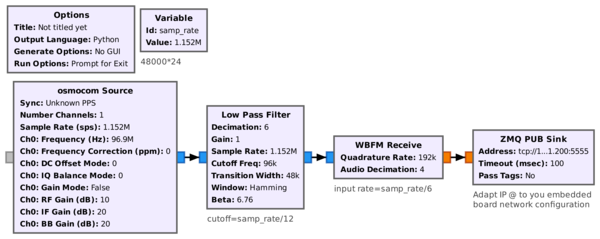
\includegraphics[width=\linewidth]{target}

Le script Python ainsi g\'en\'er\'e est transf\'er\'e \`a la RPi. Bien prendre soin
d'adapter l'adresse IP de la liaison TCP sur 0-MQ \`a l'adresse de la RPi~: le serveur
est ex\'ecut\'e sur la plateforme embarqu\'ee et en utilisant une liaison de type
Publish-Subscribe (s'apparentant \`a une liaison UDP), tout client se connectant au serveur
ex\'ecut\'e sur la cible embarqu\'ee peut recevoir le flux de donn\'ees. L'adresse IP
se incluse id\'ealement dans le sous-r\'eseau du PC pour simplifier la configuration
du routage, tandis que le port peut \^etre toute valeur au dessus de 1024. La seule
contrainte sur cette cha\^\i ne de traitement est d'aboutir \`a la fin \`a une 
fr\'equence d'\'echantillonnage \'egale \`a une valeur compatible avec la cartes son du
PC (ici 48~kHz) apr\`es une s\'equence de d\'ecimations par des facteurs entiers
s\'electionn\'ee ici par le choix d'une fr\'equence d'\'echantillonnage initiale de
$48\time 24$~kS/s. Le premier filtre passe-bas s\'electionne une unique station FM
tout en gardant assez de bande passante ($\geq$200~kHz) pour la d\'emodulation FM
\`a bande large, et le d\'emodulateur FM ajoute un second \'etage de d\'ecimation.

\section{Communication RPi vers PC}

Apr\`es traitement des donn\'ees radiofr\'equences brutes (I/Q) acquises sur la bande 
FM commerciale par la RPi, et avoir pr\'e-trait\'e le signal FM sur la plateforme
embarqu\'ee, le flux audio-fr\'equence est transmis vers le PC par 0-MQ.

\begin{center}
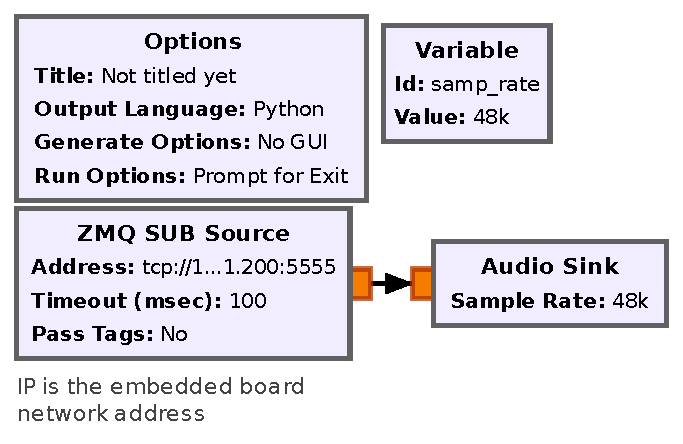
\includegraphics[width=.59\linewidth]{host}
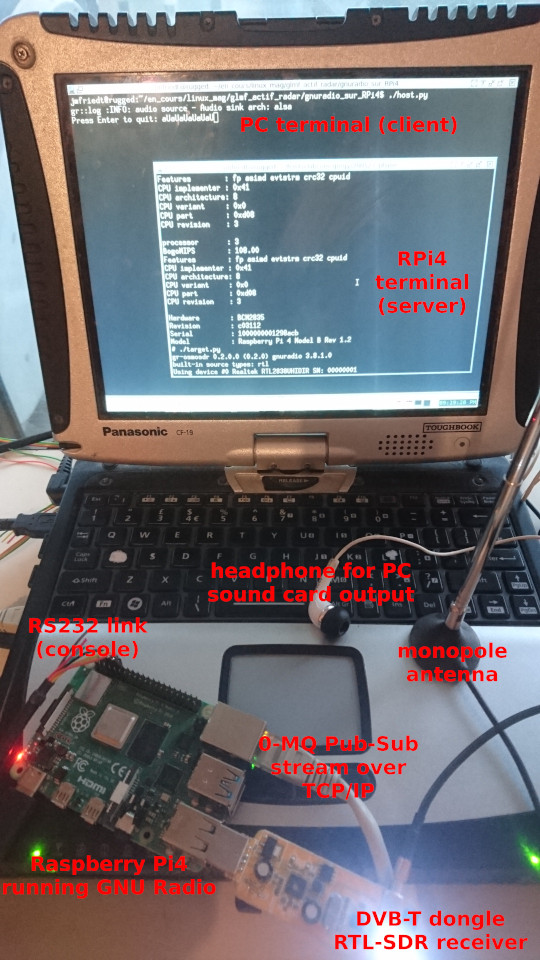
\includegraphics[width=.39\linewidth]{IMG_20200527_211928small.jpg}
\footnotesize{Gauche~: cha\^\i ne de traitement du client, qui r\'ecup\`ere un flux au format
{\em subscribe} de 0-MQ et alimente la carte son du PC. Droite~: montage exp\'erimental, 
avec une RPi4 connect\'ee par un port s\'erie virtuel et par Ethernet au PC portable. La
RPi4 \'echantillonne le flux de coefficients I/Q du r\'ecepteur de t\'el\'evision num\'erique
terrestre utilis\'e comme source de radio logicielle en ajustant sa fr\'equence dans la bande
FM, et transmet le flux audio-fr\'equence apr\`es d\'emodulation au PC, permettant d'\'ecouter
le programme gr\^ace \`a un casque connect\'e \`a la sortie de la carte son. Cette figure ne
permet pas d'illustrer l'excellente qualit\'e audio entendue \`a la sortie de la carte son,
d\'emontrant le bon fonctionnement de ce montage.}
\end{center}

\section{D\'eveloppements logiciels}

Nous nous int\'eressons \`a modifier les fonctionnalit\'es de {\tt gnss-sdr}. Le code source
de ce logiciel a \'et\'e t\'el\'echarg\'e et plac\'e dans le r\'epertoire {\tt output/build} lors
de sa s\'election et installation. Le r\'epertoire de compilation pour la cible se trouve
\`a {\tt output/build/gnss-sdr-0.0.12/buildroot-build/} tandis qu'un r\'epertoire s\'epar\'e
{\tt output/build/gnss-sdr-0.0.12/build} permet de simultan\'ement tester les modifications aux
codes sources sur le PC h\^ote. Le r\'esultat de la compilation ({\tt make}), soit dans 
{\tt buildroot-build} (cible ARM) ou {\tt build} (cible x86), se trouve dans {\tt 
src/main/gnss-sdr}.
\end{document}
